\documentclass[a4paper,12pt]{article}
\usepackage[utf8]{inputenc}
\usepackage[T1]{fontenc} 
\usepackage[french]{babel}
\usepackage{graphicx}
\usepackage{amsmath}
\usepackage{a4wide}
\usepackage{subfig}
\usepackage{wrapfig}
\usepackage{url}
\usepackage{latexsym} % \Join
\usepackage[pdftex]{hyperref}
\hypersetup{
  colorlinks,
  citecolor=black,
  filecolor=black,
  linkcolor=black,
  urlcolor=black
}
\usepackage[top=2.5cm, bottom=2.5cm, left=2cm, right=2cm]{geometry}
%\renewcommand{\baselinestretch}{1.05}

\usepackage{listings}

\lstset{ %
language=SQL,
showspaces=false
showstringspaces=false,
showtabs=false,
tabsize=2,
}

\title{INFO-H-303: projet IMDB -- seconde partie}

\author{Quentin \textsc{Stiévenart} \and Damien \textsc{Wiltgen}}
\date{\today}

\newcommand{\HRule}{\rule{\linewidth}{0.5mm}}

\begin{document}

\maketitle

\HRule

\section{Modèle entité-association}

\begin{figure}[ht!]
  \centering
  \centerline{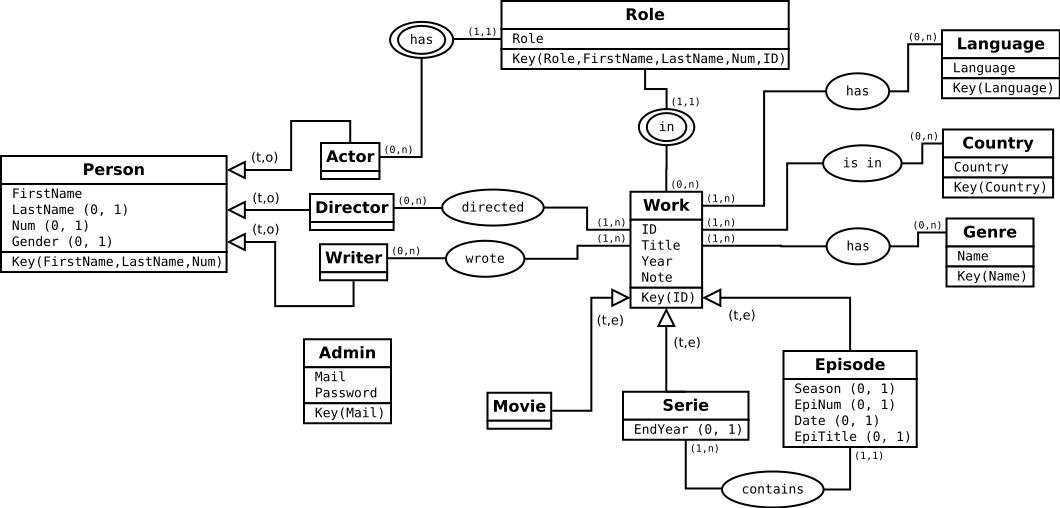
\includegraphics[width=1.1\textwidth]{er.png}}
\end{figure}

\subsection{Contraintes d'intégrité}
\begin{list}{-}{}
  \item L'année de fin d'une série doit être supérieure à son année de début.
\end{list}
\section{Modèle relationnel}
Work(\underline{ID}, Title, Year, Note)

Movie(\underline{ID})
\begin{list}{-}{}
  \item ID représente Work.ID
\end{list}

Serie(\underline{ID}, EndYear)
\begin{list}{-}{}
  \item ID représente Work.ID
\end{list}

Episode(\underline{ID}, Season, EpisodeNum, Date, EpisodeTitle, SID)
\begin{list}{-}{}
  \item ID représente Work.ID
  \item ID représente Serie.ID
\end{list}

Genre(\underline{ID, Genre})
\begin{list}{-}{}
  \item ID représente Work.ID
\end{list}

Country(\underline{ID, Country})
\begin{list}{-}{}
  \item ID représente Work.ID
\end{list}

Person(\underline{FirstName, LastName, Num}, Gender)

Actor(\underline{FirstName, LastName, Num, Role}, ID)
\begin{list}{-}{}
  \item FirstName représente Person.FirstName
  \item LastName représente Person.LastName
  \item Num représente Person.Num
  \item ID représente Work.ID
\end{list}

Writer(\underline{FirstName, LastName, Num}, ID)
\begin{list}{-}{}
  \item FirstName représente Person.FirstName
  \item LastName représente Person.LastName
  \item Num représente Person.Num
  \item ID représente Work.ID
\end{list}

Director(\underline{FirstName, LastName, Num}, ID)
\begin{list}{-}{}
  \item FirstName représente Person.FirstName
  \item LastName représente Person.LastName
  \item Num représente Person.Num
  \item ID représente Work.ID
\end{list}

Admin(\underline{Mail}, Password)
\section{Méthode d'extraction des données}
Pour extraire les données depuis les fichiers d'\emph{IMDB}, Perl a
été choisi, grâce à la facilité d'écrire des programmes manipulant du
texte ainsi qu'à la présence du module \texttt{DBI}, qui permet de
manipuler plusieurs moteurs de base de donnée en passant par une
interface unique. Il a ainsi pu être possible de tester la vitesse
d'importation de données sur plusieurs moteurs de base de données, et
le choix de moteur s'est posé sur \emph{SQLite} pour plusieurs
raisons:

\begin{list}{-}{}
  \item Les tests de contraintes étrangères sont désactivés par
    défaut, ce qui a pour effet de grandement améliorer le temps
    d'import des données. Il est possible de désactiver ces tests dans
    d'autres moteurs, mais cela dépend des moteurs et varie en
    complexité.
  \item Comme la base de donnée est simplement stockée dans un
    fichier, il est très simple de la mettre en place sur une nouvelle
    machine, d'en faire des sauvegardes, et de repartir avec une base
    de données vide.
  \item L'API \emph{SQLite} de Python (le langage utilisé pour
    l'interface web) est très simple et est fournie avec Python.
\end{list}

Pour améliorer la vitesse d'importation, les choses suivantes ont été faites:
\begin{list}{-}{}
  \item la base de donnée a été placée en RAM (dans
    \texttt{/dev/shm/}) afin de ne pas être limité par la vitesse
    d'écriture du disque dur~;
  \item le \emph{journal} de SQLite a été désactivé (\texttt{pragma
    journal\_mode = off})~;
  \item les requêtes d'insertion ont été précompilés grâce à la
    méthode \texttt{prepare}, avant d'être éxécutées un grand nombre de fois~;
  \item les transactions ont été utilisées, en désactivant
    l'\emph{AutoCommit} et en faisant un \emph{commit} à la fin de
    l'importation des données
\end{list}

Les valeurs pouvant être nulles dans le diagramme entité-associations
sont remplacées par des chaînes de caractère vides dans le cas où sont
valeurs sont des chaînes de caractères, ou par la valeur \texttt{null}
dans le cas de nombres.
\section{Requêtes demandées}
Les requêtes demandées étaient les suivantes:
\begin{list}{-}{}
  \item R1 : Les acteurs qui ont joué toutes les années entre 2003 et
    2007.
  \item R2 : Les auteurs qui ont écrit au moins deux films pendant la
    même année.
  \item R3 : Les acteurs Y qui sont à une distance 2 d'un acteur X. Un
    acteur Y est à une distance 1 d'un acteur X si ces deux acteurs
    ont joué dans le même film.
  \item R4 : Les épisodes de série où il n'y a aucun acteur masculin.
  \item R5 : Les acteurs qui ont joué dans le plus de séries.
  \item R6 : Les séries avec leur nombre total d'épisodes, le nombre
    d'épisodes moyen par an et le nombre d'acteurs moyen par saison
    depuis leur année de création et ce pour toutes les séries dont la
    note est supérieure à la moyenne des notes des séries.
\end{list}
\subsection{Algèbre relationnelle}
\begin{list}{-}{}
  \item R1 :
    \begin{align*}
      WorkInPeriod & \leftarrow \sigma_{Year \geq 2003 \wedge Year \leq 2007} (Work) \\
      AllYears & \leftarrow \pi_{Year} (WorkInPeriod)\\
      R1 & \leftarrow \pi_{FirstName, LastName, Num, Year} (Actor * WorkInPeriod) / AllYears
    \end{align*}
  \item R2 :
    \begin{align*}
      MovieWriter & \leftarrow Writer * (Work * Movie) \\
      MovieWriter' & \leftarrow \alpha_{ID,Title:ID2,Title2} (MovieWriter) \\
      R2 & \leftarrow \pi_{FirstName,LastName,Num} (MovieWriter \Join_{ID \neq ID2 \wedge Title \neq Title2} MovieWriter')
    \end{align*}
  \item R3 :
    Si les infos sur l'acteur X sont dans $XFName$, $XLName$, $XNum$
    \begin{align*}
      X & \leftarrow \sigma_{FirstName = XFName \wedge LastName = XLName \wedge Num = XNum} (Actor) \\
      R3 & \leftarrow \pi_{FirstName,LastName,Num}(Actor*\pi_{ID} (X * (Work * Movie))
    \end{align*}
  \item R4 :
    \begin{align*}
      R4 & \leftarrow \pi_{ID} (Episodes) - \pi_{ID} ((\sigma_{Gender='M'} Person) * Actor * Episode)
    \end{align*}
\end{list}
\subsection{Calcul relationnel tuple}
\begin{list}{-}{}
  \item R1 :
    \begin{align*}
    \{ a.FirstName, a.LastName, a.Num | &Actor(a) \wedge \exists w1, w2, w3, w4, w5 ( \\
    &Work(w1) \wedge w1.ID = a.ID \wedge w1.Year = 2003 \wedge \\
    &Work(w2) \wedge w2.ID = a.ID \wedge w2.Year = 2004 \wedge \\
    &Work(w3) \wedge w3.ID = a.ID \wedge w3.Year = 2005 \wedge \\
    &Work(w4) \wedge w4.ID = a.ID \wedge w4.Year = 2006 \wedge \\
    &Work(w5) \wedge w5.ID = a.ID \wedge w5.Year = 2007)\}
    \end{align*}
  \item R2 :
    \begin{align*}
      \{ a1.FirstName, a1.LastName, a1.Num | &Writer(a1) \\
      \wedge \exists w1, w2, a2, f1, f2 ( \\
      &Work1(w1) \wedge Work2(w2) \wedge Writer(a2) \wedge Movie(f1) \wedge Movie(f2) \\
      \wedge &w1.ID = f1.ID \wedge w1.ID = a1.ID
      \wedge &w2.ID = f2.ID \wedge w2.ID = a2.ID
      \wedge &a1.FirstName = a2.FirstName \wedge a1.LastName = a2.LastName \\
      \wedge &a1.Num = a2.Num \\
      \wedge &w2.Year = w1.Year \\
      \wedge &w2.ID \neq w1.ID ) \}
    \end{align*}
  \item R3 :
    Si les infos sur l'acteur X sont dans $XFName$, $XLName$, $XNum$
    \begin{align*}
      \{ x.FirstName, x.LastName, x.Num | &Actor(x) \wedge \exists y_1, y_2, z ( \\
      &Actor(z) \wedge Actor(y_1) \wedge Actor(y_2) \wedge \\
      &y_1.ID = x.ID \wedge y_2.ID = z.ID \wedge y_1.ID \neq y_2.ID \wedge\\
      &y_1.FirstName = y_2.FirstName \wedge \\
      &y_1.LastName = y_2.LastName \wedge \\
      &y_1.Num = y_2.Num) \wedge \\
      &z.FirstName = XFName \wedge z.LastName = XLName \wedge \\
      &z.Num = XNum\}
    \end{align*}
  \item R4 :
    \begin{align*}
      \{ e.ID | Episode(e) \wedge \lnot \exists p, a (&Person(p) ~\wedge Actor(a) ~\wedge \\
        & p.FirstName = a.FirstName ~\wedge \\
        & p.LastName = a.LastName ~\wedge \\
        & p.Num = a.Num ~\wedge \\
        & p.Gender = `M`)\}
    \end{align*}
\end{list}
          
\subsection{SQL}
\begin{list}{-}{}
  \item R1 :
    \begin{lstlisting}
select FirstName, LastName, Num from Actor where
  count(select distinct(Year) from Work
          where Year >= 2003 
            and Year <= 2007
            and Actor.ID = Work.ID) = (2007-2003)

    \end{lstlisting}
  \item R2 :
    \begin{lstlisting}
select distinct FirstName, LastName, Num
  from Writer, Movie, Work
  where Writer.ID=Movie.ID and Work.ID=Movie.ID
  group by FirstName, LastName, Num, Year
  having count(Writer.ID) >= 2
    
    \end{lstlisting}
  \item R3 :
    Si les infos sur l'acteur X sont dans $XFName$, $XLName$, $XNum$
    \begin{lstlisting}
select distinct X.FirstName, X.LastName, X.Num from Actor X
  where exists (select * from Actor Y1
                  where exists (select * from Actor Z, Actor Y2 
                                  where Z.ID = Y2.ID
                                    and Z.ID != X.ID
                                    and Z.FirstName = ZFName
                                    and Z.LastName = ZLName
                                    and Z.Num = ZNum
                                    and Y2.FirstName = Y1.FirstName
                                    and Y2.LastName = Y1.LastName
                                    and Y2.Num = Y1.Num)
                    and Y1.ID = X.ID)
    \end{lstlisting}
  \item R4 :
    \begin{lstlisting}
select ID from Episode
  where not exists (select * from Person, Actor
                      where Person.FirstName = Actor.FirstName
                        and Person.LastName = Actor.LastName
                        and Person.Num = Actor.Num
                        and Actor.ID = Episode.ID)
    \end{lstlisting}
  \item R5 :
    \begin{lstlisting}
select FirstName, LastName, Num, count(*) as compteur
  from Actor, Serie
  where Actor.ID=Serie.ID
  group by FirstName,LastName,Num
  order by compteur desc
    \end{lstlisting}
  \item R6 :
    % TODO
    \begin{lstlisting}
SELECT COUNT(E.ID),
  COUNT(E.ID)/(2011 - W1.Year + 1 + (SELECT EndYear - 2011
                                     FROM Serie S4
                                     WHERE S4.ID=S1.ID)),
  (SELECT COUNT(*)
   FROM Actor
   WHERE Actor.ID=S1.ID)
       
  FROM Episode E, Serie S1, Work W1
  WHERE E.SID=S1.ID AND W1.ID=S1.ID AND W1.Note > (SELECT AVG(Note)
                                                   FROM Work W3, Serie S3
                                                   WHERE S3.ID=W3.ID)
  GROUP BY E.SID;
    \end{lstlisting}
\section{Hypothèses}
\section{Interface}
Afin de consulter les données, une interface web a été développée en
Python, en utilisant les technologies suivantes:
\begin{list}{-}{}
  \item \emph{Tornado} comme serveur web, ainsi que module de templates~;
  \item \emph{SQLite 3} pour manipuler la base de donnée~;
  \item \emph{Lex} et \emph{Yacc} pour parser le langage de recherche.
\end{list}

Outre la base demandée, les fonctionnalitées suivantes ont été développées:
\begin{list}{-}{}
  \item Un langage de recherche permettant de faire des recherches évoluées
  \item La localisation des films sur une carte \emph{Google Maps}
  \item L'affichage du poster des films, en utilisant
    \texttt{http://imdbapi.com} pour récupérer les URL des images
  \item Un système de vote à la \emph{Reddit} (chaque visiteur peut
    \emph{upvoter} ou \emph{downvoter} une œuvre)
\end{list}

\end{list}

\end{document}
